\documentclass[border=10pt]{standalone}
\usepackage{tikz}
\usetikzlibrary{shapes.geometric,arrows.meta,positioning,calc}
\definecolor{cwork}{RGB}{72,116,158}
\definecolor{csetup}{RGB}{86,156,104}
\definecolor{crepair}{RGB}{198,86,76}
\begin{document}
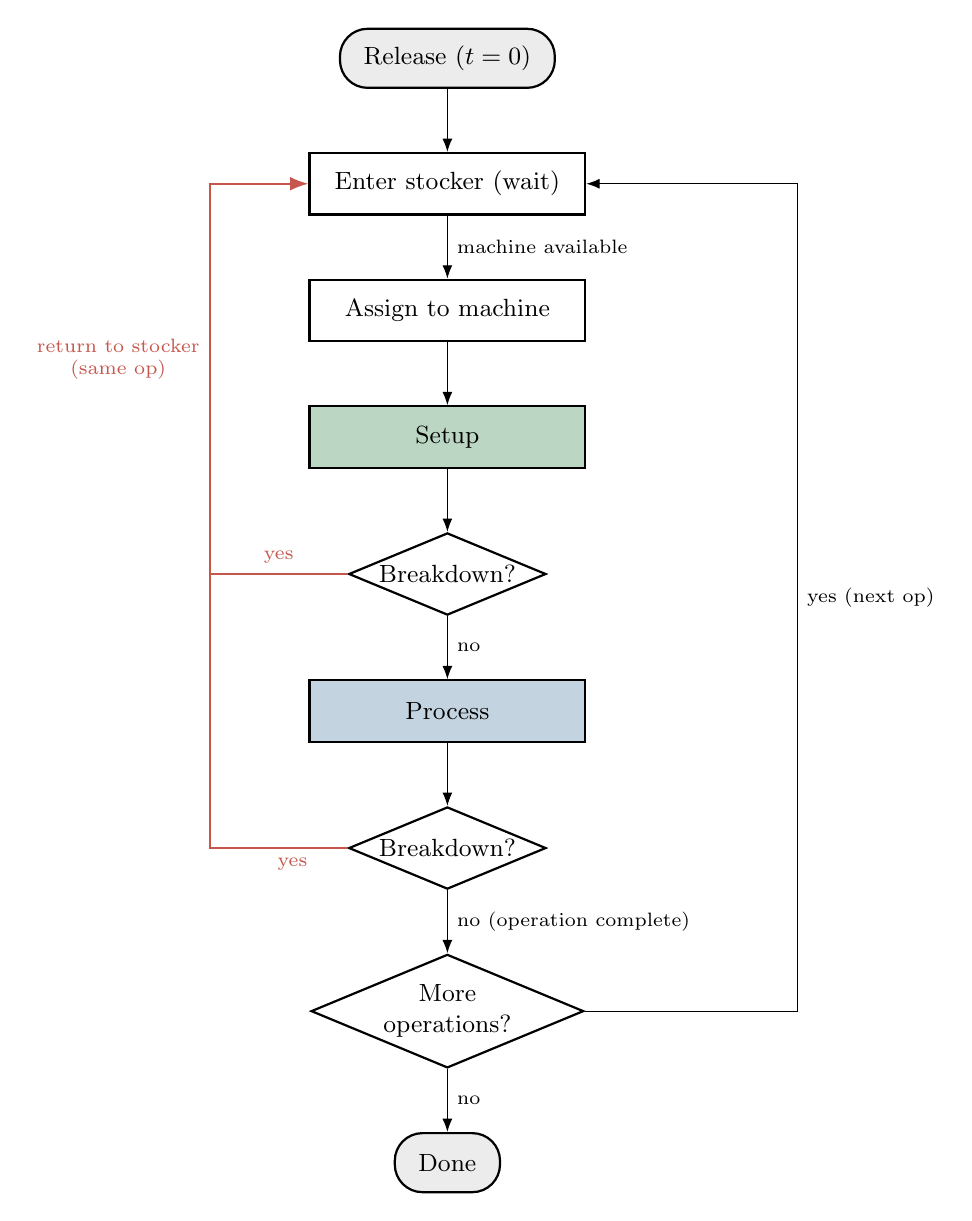
\begin{tikzpicture}[font=\small,>=Latex,node distance=0.8cm,
  term/.style={draw,thick,rounded corners=10pt,fill=gray!15,minimum height=0.75cm,inner xsep=3mm,align=center},
  act/.style={draw,thick,minimum width=3.5cm,minimum height=0.78cm,align=center},
  dec/.style={diamond,draw,thick,aspect=2.4,inner sep=1pt,align=center,fill=white}]
  \node[term] (start) {Release ($t=0$)};
  \node[act,below=of start] (stk) {Enter stocker (wait)};
  \node[act,below=of stk] (assign) {Assign to machine};
  \node[act,fill=csetup!40,below=of assign] (setup) {Setup};
  \node[dec,below=of setup] (brk1) {Breakdown?};
  \node[act,fill=cwork!32,below=of brk1] (proc) {Process};
  \node[dec,below=of proc] (brk2) {Breakdown?};
  \node[dec,below=of brk2] (more) {More\\operations?};
  \node[term,below=of more] (done) {Done};
  \coordinate[left=1.75cm of brk1] (failhub);
  \coordinate (stockerReturn) at (failhub |- stk.west);
  \draw[->] (start)--(stk);
  \draw[->] (stk)-- node[right,font=\scriptsize]{machine available} (assign);
  \draw[->] (assign)--(setup);
  \draw[->] (setup)--(brk1);
  \draw[->] (brk1)-- node[right,font=\scriptsize]{no} (proc);
  \draw[->] (proc)--(brk2);
  \draw[->] (brk2)-- node[right,font=\scriptsize]{no (operation complete)} (more);
  \draw[->] (more)-- node[right,font=\scriptsize]{no} (done);
  \draw[crepair,thick] (brk1.west) -- node[above,font=\scriptsize]{yes} (failhub);
  \draw[crepair,thick] (brk2.west) -| node[below,font=\scriptsize,pos=0.2]{yes} (failhub);
  \draw[->,crepair,thick] (failhub)
    -- node[left,font=\scriptsize,align=center,pos=0.55]{return to stocker\\(same op)} (stockerReturn)
    -- (stk.west);
  \draw[->] (more.east) -- ++(2.7,0) |- node[right,font=\scriptsize,pos=0.25]{yes (next op)} (stk.east);
\end{tikzpicture}
\end{document}
